\chapter{Search for Resonant Di-Higgs }
\label{ch:diHiggs_search}

% \chapter{Search for Resonant Di-Higgs Production in the \texorpdfstring{\(X \to HH \to WW\gamma\gamma\)}{X->HH->WWgg} Channel}

\section{Introduction and Motivation}
The study of Higgs boson pair production provides a unique opportunity to probe the Higgs self-coupling and to search for physics
beyond the Standard Model (BSM). In the SM, Higgs boson pairs are dominantly produced via gluon-gluon fusion (ggF) through triangle
and box diagrams, as shown in Fig.~\ref{SMLO_ggHH_production}, that exhibit destructive interference.
The predicted cross section for non-resonant di-Higgs production is small, \(0.01449 \pm 0.000019\)~pb,
making this process challenging to observe.
\begin{figure}[!htbp]
    \begin{center}
        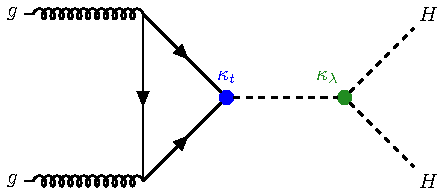
\includegraphics[width=0.45\textwidth]{figures/diHiggsSearches/fey_HH_Triangle.pdf} %
        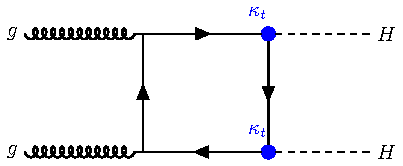
\includegraphics[width=0.45\textwidth]{figures/diHiggsSearches/fey_HH_Box.pdf}
    \end{center}
    \caption{Feynman diagrams for leading-order Higgs boson pair production via gluon fusion}
    \label{SMLO_ggHH_production}
\end{figure}
\begin{figure}[!htbp]
    \begin{center}
        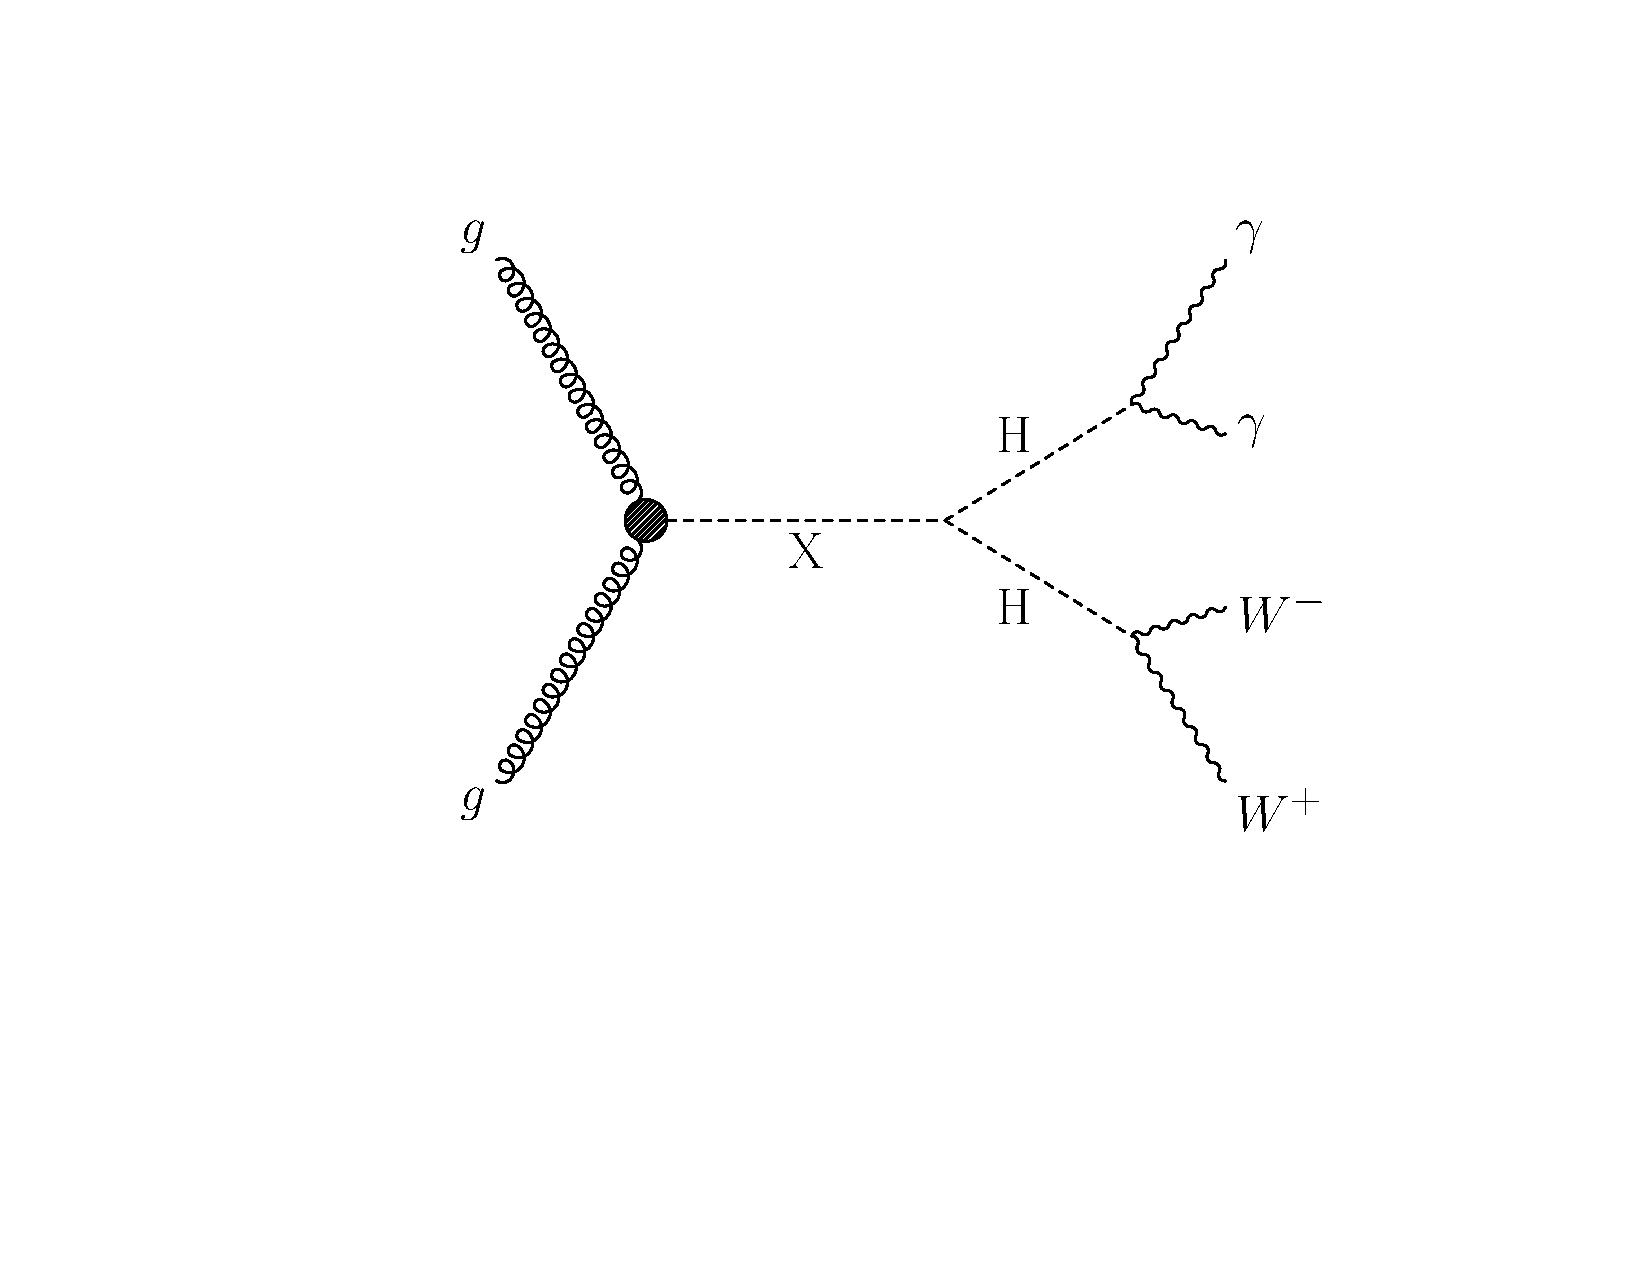
\includegraphics[width=0.45\textwidth]{figures/diHiggsSearches/fey_XHH_HHWWgg.pdf}
    \end{center}
    \caption{Feynman diagram for resonant di-Higgs production in the \HH channel}
    \label{XHHFeynmanDiagram}
\end{figure}


Extensions of the SM, such as the Next-to-Minimal Supersymmetric Standard Model (NMSSM), Randall-Sundrum models, or the two-Higgs
doublet model (2HDM), predict resonant di-Higgs production. In these scenarios, a heavy resonance \(X\) decays into two Higgs
bosons, which subsequently decay into \(WW\) and \(\gamma\gamma\), as shown in Fig.~\ref{XHHFeynmanDiagram}. This analysis specifically focuses on \(X \to HH \to
WW\gamma\gamma\), leveraging the clean diphoton final state to enhance sensitivity while covering all possible jet topologies.


\section{Analysis Overview}
The analysis is performed using the full Run-2 Ultra-Legacy dataset, corresponding to an integrated luminosity of 138~fb\(^{-1}\) at
\(\sqrt{s} = 13\)~TeV. The following decay channels are explored:
\begin{itemize}
    \item \textbf{Semi-leptonic (\(l\nu qq\gamma\gamma\)):} One \(W\) boson decays leptonically (\(W \to l\nu\)), and the other
    decays hadronically (\(W \to qq\)).
    \item \textbf{Fully hadronic (\(4q\gamma\gamma\)):} Both \(W\) bosons decay hadronically (\(W \to qq\)).
\end{itemize}

\section{Unique Features of the Analysis}
This analysis incorporates several innovative aspects, as detailed below:

\begin{itemize}
    \item \textbf{Comprehensive Topology Coverage:}
    For the first time, all jet topologies are tagged within a single analysis. These include boosted, semi-boosted, resolved, and scenarios where leptons are reconstructed inside jets.

    \item \textbf{Signal Definition:}
    The signal is defined as the sum of three di-Higgs decay possibilities:
    \[
    HH \to WW\gamma\gamma + ZZ\gamma\gamma + bb\gamma\gamma.
    \]
    Since the hadronic decay topologies are similar for all three channels, it is challenging to reduce contamination from the \(ZZ\gamma\gamma\) and \(bb\gamma\gamma\) channels in our primary signal of interest, \(WW\gamma\gamma\). The signal definition is further refined with the following considerations:
    \begin{itemize}
        \item The analysis is optimized for the \(HH \to WW\gamma\gamma\) channel.
        \item For \(HH \to WW\gamma\gamma\), two decay modes of the \(W\)-bosons are considered: fully hadronic and semi-leptonic. The analysis optimization is performed based on these two final states.
        \item For \(HH \to ZZ\gamma\gamma\), due to the low branching fraction and negligible semi-leptonic contribution, the semi-leptonic decay mode is excluded from the analysis.
        \item The \(bb\gamma\gamma\) channel is included after applying a b-jet veto. This serves multiple purposes:
        \begin{enumerate}
            \item It reduces the contribution from the \(bb\gamma\gamma\) channel, ensuring that the limit is primarily driven by the \(WW\gamma\gamma\) channel rather than \(bb\gamma\gamma\).
            \item It makes the analysis orthogonal to the \(HH \to bb\gamma\gamma\) analysis.
            \item Events rejected by the \(HH \to bb\gamma\gamma\) analysis are exploited, thereby utilizing additional information from the same dataset.
            \item The b-jet veto also rejects events from \(HH \to ZZ\gamma\gamma\) where the \(Z\)-bosons decay into b-quarks.
        \end{enumerate}
    \end{itemize}

    \item \textbf{Mass Ranges:}
    The resonance \(X\) is studied over a mass range of 250~GeV to 3000~GeV.

    \item \textbf{Leptons Inside Jets:}
    Events where leptons are reconstructed within jets are included, thereby enhancing sensitivity to specific Beyond Standard Model (BSM) scenarios.
\end{itemize}

\section{Event Selection}


The event selection optimizes sensitivity to semi-leptonic and fully hadronic channels, with the following criteria:

\subsection*{Photon Selection}
\begin{itemize}
    \item A boosted decision tree (BDT) classifier is trained to separate photons from jets~\cite{Sirunyan:2018ouh}.
            The output of this BDT is referred to as the photon ID score
            \footnote{For the boosted regime, where the two photons are close by, the photon ID score was modified to
            account for reduced selection efficiency.
            This modified score is referred to as the ``modified photon ID," detailed in
            Appendix~\ref{appendix:ModifiedPhotonID}}.
    \item Leading photon \(p_T > 35\)~GeV and subleading photon \(p_T > 25\)~GeV.
    \item Photon transverse momentum fractions: \(p_T/m_{\gamma\gamma} > 0.33\) (leading) and \(> 0.25\) (subleading).
    \item Diphoton invariant mass requirement: \(100 < m_{\gamma\gamma} < 180\)~GeV.
\end{itemize}


\subsection*{Lepton Selection}
\begin{itemize}
    \item \todo[inline]{Missing the ID for isolated as well as non-isolated leptons}
    \item Isolated leptons: \(p_T > 10\)~GeV, \(|\eta| < 2.4\), with \(\Delta R(l,\gamma) > 0.4\)
    \item Non-isolated leptons: \(\Delta R(l, \text{FatJet}) < 0.8\), with relaxed isolation criteria.
    \item \(Z\)-veto: \(|m_{l\gamma} - 91.2| > 5\)~GeV to suppress \(Z\)-boson contamination.
\end{itemize}

\subsection*{Jet Selection}
\begin{itemize}
    \item AK4 jets: \(p_T > 30\)~GeV, \(|\eta| < 2.4\), passing tight jet ID \todo[inline]{Define ID}.
    \item AK8 jets: \(p_T > 200\)~GeV, \(|\eta| < 2.4\), with jet mass consistent with \(W\)- or Higgs-like jets.
    \item Boosted Higgs tagging uses ParticleNet \todo[inline]{define particleNet in the footnote} with a score threshold of 0.2.
\end{itemize}

\subsection*{Event Topologies}
Four jet categories are defined:
\begin{itemize}
    \item \textbf{1-jet:} A single AK8 jet tagged as a Higgs jet.
    \item \textbf{2-jet:} Two AK8 jets, one tagged as a Higgs jet and the other as a \(W\)-jet.
    \item \textbf{3-jet:} One AK8 jet combined with two AK4 jets.
    \item \textbf{4-jet:} Fully resolved topology with four AK4 jets.
\end{itemize}


\section{Data-Driven Background Estimation}
Accurate estimation of backgrounds is crucial for isolating the signal in the \(X \to HH \to WW\gamma\gamma\) analysis.
The dominant backgrounds include non-resonant diphoton production, single Higgs processes, and multijet events
where fake photons mimic the signal.
A data-driven strategy is employed to estimate fake photon backgrounds, inspired by CMS analysis HIG-19-013.

\subsection{Motivation}
The low statistics of QCD Monte Carlo (MC) samples result in poor modeling of important input features to multivariate analyses. To
ensure agreement between data and MC and unbiased training of machine learning models, a data-driven approach is adopted. The method
uses events from the photon ID MVA sideband to model fake photon contributions.

\subsection{Methodology}
The following steps outline the data-driven background estimation strategy:

\begin{enumerate}
    \item \textbf{Photon ID Sideband Selection:}
    Events that fail the preselection cut on the photon ID MVA are used to model fake photons. The sideband regions are chosen as:
    \begin{itemize}
        \item Resolved category: Minimum photon ID MVA in the range \([-0.9, -0.7]\),
        \item Boosted category: Minimum photon ID MVA in the range \([-0.95, -0.9]\).
    \end{itemize}

    \item \textbf{PDF Generation for Fake Photons:}
    A probability density function (PDF) for the photon ID MVA distribution of fake photons is obtained from MC samples (e.g.,
    \(\gamma + \text{jets}\)). The sideband events are reweighted to match the fake photon PDF in the signal region.

    \item \textbf{Reweighting and Normalization:}
    Events in the photon ID sideband are assigned per-event weights to reshape the maximum photon ID MVA distribution. The weight
     \(w\) is defined as:
    \begin{equation}
        w = \frac{\int_{\text{minID}}^{\text{maxID}} \text{fakePDF}(x) \, dx}
                 {\int_{\text{sidebandMinID}}^{\text{sidebandMaxID}} \text{fakePDF}(x) \, dx}.
    \end{equation}
    Different weight functions are applied for resolved and boosted categories.

    \item \textbf{Validation:}
    The reweighted MC is normalized to data to ensure consistency. Comparisons before and after applying the data-driven method demonstrate improved agreement in key variables, such as \(m_{\gamma\gamma}\).
\end{enumerate}

\subsection{Challenges and Solutions}
The data-driven method is validated for both fully hadronic (FH) and semi-leptonic (SL) channels. However, specific challenges arise:
\begin{itemize}
    \item \textbf{Muon Channel in SL Events:}
    While the method improves data-MC agreement in the electron channel, it worsens agreement in the muon channel. Possible solutions include:
    \begin{itemize}
        \item Use the data-driven approach for the electron channel only.
        \item Perform separate reweighting for the electron and muon channels.
    \end{itemize}
    Currently, a combined reweighting technique is applied to correct control plots, ensuring consistent results without relying
    heavily on MC samples.

    \item \textbf{Photon ID Sidebands:}
    Assumptions underlying the sideband method include:
    \begin{enumerate}
        \item Other variables used in the analysis are minimally correlated with the photon ID MVA.
        \item The low photon ID sideband is dominated by fake photons (e.g., from QCD and \(\gamma + \text{jets}\)).
        \item Photons in the low ID sideband are always fake.
    \end{enumerate}
\end{itemize}

\subsection{Implementation in Different Channels}
The method is applied to both fully hadronic and semi-leptonic channels:
\begin{itemize}
    \item \textbf{Fully Hadronic Channel:}
    Dominated by QCD backgrounds, where the photon ID MVA sideband reliably models fake photon contributions.
    \item \textbf{Semi-Leptonic Channel:}
    Includes fake photon contributions from \(W\gamma\gamma\) and \(t\bar{t}\) processes, with non-isolated leptons contributing to
    the final background estimation.
\end{itemize}

\subsection{Impact of the Data-Driven Method}
The results of the data-driven background estimation are as follows:
\begin{itemize}
    \item Significant improvement in the modeling of photon-related variables in both resolved and boosted categories.
    \item Enhanced agreement between data and MC distributions in control regions, as shown in Figure~\ref{fig:control_plots}.
    \item Improved sensitivity to the \(X \to HH \to WW\gamma\gamma\) signal, particularly in high-mass regions.
\end{itemize}

The control plots for the resolved and boosted regions before and after applying the data-driven method demonstrate the
effectiveness of this strategy. Future improvements will address challenges in the muon channel and refine the photon ID sideband
methodology.

\section{Multivariate Analysis Using Parameterized Neural Network (pNN)}

To maximize the sensitivity of the search for resonant \(X \to HH \to WW\gamma\gamma\), a multivariate analysis (MVA) is performed
using a Parameterized Neural Network (pNN). The pNN method allows for simultaneous training across multiple signal hypotheses,
parameterized by the mass of the heavy resonance \(m_X\). This approach ensures a more robust discrimination between signal and
background across a wide range of masses, from 250~GeV to 3000~GeV.

\subsection{Overview of pNN Methodology}
The pNN method is implemented as a deep feed-forward neural network. The network inputs include kinematic and topological features of the events, while the resonance mass \(m_X\) is used as a parameter to generalize the signal hypothesis. The key features of the pNN method are:
\begin{itemize}
    \item \textbf{Parameterized Mass Input:} The network is trained with the resonance mass \(m_X\) as an input variable, enabling simultaneous training for multiple signal mass points.
    \item \textbf{Dropout Layer:} Introduced to prevent overtraining and enhance generalization.
    \item \textbf{Optimizer:} The Adam optimizer is used for training with stochastic gradient descent.
    \item \textbf{GPU-Based Training:} Training is accelerated using GPUs for efficient processing of large datasets.
\end{itemize}

\subsection{Training Strategy}
Separate pNNs are trained for the **boosted** and **resolved** topologies due to the distinct event kinematics in these categories:
\begin{itemize}
    \item \textbf{Boosted Category:} Events where \(W\)-bosons' decay products are merged into single AK8 jets.
    \item \textbf{Resolved Category:} Events where \(W\)-bosons' decay products are reconstructed as individual AK4 jets.
\end{itemize}

The input features for the pNN are selected based on their ability to discriminate signal from background. These features include photon, jet, and missing transverse energy (\(E_T^{\text{miss}}\)) observables.

\subsection{Input Features}
The key input variables used for training the pNN are listed in Tables~\ref{tab:pnn_boosted_inputs} and \ref{tab:pnn_resolved_inputs}.

\begin{table}[h!]
    \centering
    \caption{Input variables for the pNN in the boosted category.}
    \label{tab:pnn_boosted_inputs}
    \begin{tabular}{ll}
        \hline
        \textbf{Feature} & \textbf{Description} \\
        \hline
        Diphoton \(p_T/m_{\gamma\gamma}\) & Transverse momentum of diphoton system normalized to \(m_{\gamma\gamma}\) \\
        Diphoton \(dR\) & Angular separation between leading and subleading photons \\
        Leading Photon \(p_T/m_{\gamma\gamma}\) & Leading photon \(p_T\) normalized to \(m_{\gamma\gamma}\) \\
        Subleading Photon \(p_T/m_{\gamma\gamma}\) & Subleading photon \(p_T\) normalized to \(m_{\gamma\gamma}\) \\
        FatJet \(p_T\), \(m\), \(\eta\), \(\phi\) & Transverse momentum, mass, pseudorapidity, and azimuthal angle of leading AK8 jets \\
        \(E_T^{\text{miss}}\) & Missing transverse energy \\
        FatJet-diphoton \(dR\) & Angular separation between leading fatjet and diphoton system \\
        \hline
    \end{tabular}
\end{table}

\begin{table}[h!]
    \centering
    \caption{Input variables for the pNN in the resolved category.}
    \label{tab:pnn_resolved_inputs}
    \begin{tabular}{ll}
        \hline
        \textbf{Feature} & \textbf{Description} \\
        \hline
        Diphoton \(p_T/m_{\gamma\gamma}\) & Transverse momentum of diphoton system normalized to \(m_{\gamma\gamma}\) \\
        Diphoton \(dR\) & Angular separation between leading and subleading photons \\
        Leading Jet \(p_T\), \(m\), \(\eta\), \(\phi\) & Kinematic properties of leading AK4 jets \\
        Subleading Jet \(p_T\), \(m\), \(\eta\), \(\phi\) & Kinematic properties of subleading AK4 jets \\
        Diphoton-jet \(dR\) & Angular separation between diphoton system and jets \\
        \(E_T^{\text{miss}}\) & Missing transverse energy \\
        B-jet Scores & Highest and second-highest b-tagging scores for AK4 jets \\
        \hline
    \end{tabular}
\end{table}

\subsection{Performance and Validation}
The performance of the pNN is validated using standard metrics such as the area under the curve (AUC) and signal-to-background ratio improvements. The following observations are noted:
\begin{itemize}
    \item The pNN significantly enhances discrimination between signal and background across the entire mass range.
    \item Feature importance plots indicate that the most discriminating variables are the diphoton \(p_T/m_{\gamma\gamma}\), \(dR\) between photons, and jet kinematics.
    \item Separate training for the boosted and resolved categories optimizes sensitivity in their respective regions.
\end{itemize}

\subsection{Results of the pNN Classification}
The output of the pNN is used as the final discriminant to extract the signal in the \(m_{\gamma\gamma}\) distribution. By combining the boosted and resolved topologies, the analysis achieves a 60\% improvement in sensitivity over previous results.

\subsection{Summary of pNN Method}
The parameterized neural network approach provides a powerful method for signal extraction in the \(X \to HH \to WW\gamma\gamma\) analysis. By training across multiple mass hypotheses and incorporating advanced multivariate techniques, the pNN significantly improves the sensitivity to resonant di-Higgs production.

\section{Results}
Results are interpreted in terms of cross-section limits on \(X \to HH \to WW\gamma\gamma\). Key outcomes include:
\begin{itemize}
    \item At \(m_X = 3000\)~GeV, the observed (expected) limit is 60~fb for \(X \to HH \to WW\gamma\gamma\).
    \item The analysis shows a 60\% improvement in sensitivity compared to ATLAS at 500~GeV.
    \item Incorporating leptons inside jets enhances sensitivity, particularly in semi-leptonic topologies.
\end{itemize}

\section{Systematic Uncertainties}
Major systematic uncertainties include:
\begin{itemize}
    \item QCD scale variations for high-mass resonances.
    \item Photon energy resolution and identification efficiency.
    \item Jet energy scale and resolution.
\end{itemize}

The impact of these uncertainties is quantified and incorporated into the statistical interpretation.

\section{Signal and Background Modelling}
\label{sec:signal_background_modelling}

The extraction of the \(X \to HH \to WW\gamma\gamma\) signal is performed using the same methodology as the Higgs boson analysis in the \(H \to \gamma\gamma\) channel~\cite{CMS:2020xrn}. This involves precise modelling of the signal shape using simulated samples and the background shape using data-driven techniques.

\subsection{Signal Modelling}
The signal shape is parameterized based on Monte Carlo (MC) simulations, with the diphoton invariant mass \(m_{\gamma\gamma}\) as the primary observable.

\begin{itemize}
    \item \textbf{Signal Simulation:}
    \begin{itemize}
        \item Signal samples are generated at leading order (LO) using \textsc{MadGraph5\_aMC@NLO} for the gluon-gluon fusion process \(gg \to X\).
        \item Subsequent parton showering and hadronization are performed with \textsc{Pythia8}, and detector effects are simulated using the CMS \textsc{Geant4}-based framework.
        \item Simulated samples are produced for resonance masses \(m_X\) ranging from 250~GeV to 3000~GeV.
    \end{itemize}

    \item \textbf{Signal Shape:}
    \begin{itemize}
        \item The diphoton mass distribution for the signal is modelled using a double-sided Crystal Ball (CB) function, defined as:
        \[
        f_{\text{CB}}(x) =
        \begin{cases}
            A \exp\left(-\frac{(x-\mu)^2}{2\sigma^2}\right), & \text{for } |x-\mu| \leq \alpha\sigma, \\
            B \left(\frac{n}{\alpha} - \frac{n}{\alpha - (x-\mu)/\sigma} \right)^{-n}, & \text{for } x-\mu > \alpha\sigma,
        \end{cases}
        \]
        where \(\mu\) is the mean, \(\sigma\) is the width, and \(\alpha\), \(n\) define the tail parameters.
        \item The parameters of the Crystal Ball function are extracted from fits to the MC simulation in each analysis category (boosted and resolved).
        \item The normalization of the signal is determined from the integrated luminosity and the predicted cross section for \(X \to HH \to WW\gamma\gamma\).
    \end{itemize}

    \item \textbf{Signal Categories:}
    The analysis is divided into multiple categories to maximize sensitivity:
    \begin{itemize}
        \item \textbf{Boosted:} Events where the \(W\)-boson decay products are merged into single large-radius jets.
        \item \textbf{Resolved:} Events where the \(W\)-boson decay products are reconstructed as separate small-radius jets.
        \item \textbf{Semi-leptonic and fully hadronic:} These subcategories depend on the final-state reconstruction of leptons or jets.
    \end{itemize}
\end{itemize}

\subsection{Background Modelling}
The dominant background arises from SM non-resonant diphoton production, with additional contributions from single Higgs production and fake photon processes. The background is modelled using the following approaches:

\begin{enumerate}
    \item \textbf{Non-Resonant Diphoton Background:}
    \begin{itemize}
        \item The continuum diphoton background is modelled directly from data using a smooth analytic function. This function is chosen based on its ability to fit the diphoton invariant mass sidebands while avoiding bias in the signal region.
        \item A range of functional forms, such as exponentials, power laws, or Bernstein polynomials, is tested. The optimal choice is selected using the Fisher F-test and evaluated for bias using pseudo-experiments.
        \item The background shape parameters are determined from fits to the \(m_{\gamma\gamma}\) sideband regions (\(100 < m_{\gamma\gamma} < 120\)~GeV and \(130 < m_{\gamma\gamma} < 180\)~GeV).
    \end{itemize}

    \item \textbf{Resonant Backgrounds:}
    \begin{itemize}
        \item Single Higgs production (\(ggH\), VBF, \(VH\)) with \(H \to \gamma\gamma\) is a subdominant but irreducible background. It is modelled using MC simulation normalized to the theoretical cross sections.
        \item Other rare processes such as \(t\bar{t}\gamma\gamma\), \(W\gamma\gamma\), and \(Z\gamma\gamma\) are also estimated from MC samples.
    \end{itemize}

    \item \textbf{Fake Photon Background:}
    \begin{itemize}
        \item Events where jets or electrons are misidentified as photons are estimated using a data-driven method based on the photon ID MVA sideband technique (Section~\ref{sec:data_driven_bkg}).
        \item The contribution of fake photons is validated in control regions enriched with QCD multijet events.
    \end{itemize}
\end{enumerate}

\subsection{Systematic Uncertainties}
The systematic uncertainties affecting the signal and background modelling include:
\begin{itemize}
    \item \textbf{Signal Modelling:}
    \begin{itemize}
        \item Uncertainty in the Crystal Ball function parameters.
        \item Theoretical uncertainties in the signal cross section due to renormalization and factorization scales.
    \end{itemize}
    \item \textbf{Background Modelling:}
    \begin{itemize}
        \item Uncertainties in the choice of the analytic function for the non-resonant background.
        \item Statistical uncertainties in the fits to sideband data.
    \end{itemize}
    \item \textbf{Experimental Uncertainties:}
    \begin{itemize}
        \item Photon energy scale and resolution uncertainties.
        \item Jet energy scale (JES) and jet energy resolution (JER) uncertainties.
        \item Integrated luminosity uncertainty of 1.6\%.
    \end{itemize}
\end{itemize}

\subsection{Result Extraction}
The signal extraction is performed using an unbinned maximum likelihood fit to the diphoton invariant mass spectrum \(m_{\gamma\gamma}\) in each analysis category. The signal and background components are parameterized as:
\[
f_{\text{total}}(m_{\gamma\gamma}) = N_{\text{sig}} f_{\text{sig}}(m_{\gamma\gamma}) + N_{\text{bkg}} f_{\text{bkg}}(m_{\gamma\gamma}),
\]
where \(f_{\text{sig}}\) is the signal shape modelled by the Crystal Ball function, and \(f_{\text{bkg}}\) is the smooth analytic function for the non-resonant background.

The parameters \(N_{\text{sig}}\) and \(N_{\text{bkg}}\) are extracted simultaneously through the likelihood fit, with systematic uncertainties incorporated as nuisance parameters.


\section{Signal and background modelling} \label{sec:AnalyticFitting}

In order to model the di-Higgs signal process, and single higgs resonant background processes in the signal region, 115 $< \mgg < $ 135 GeV, simulated events
in each analysis category are combined to construct $\mgg$ shapes. Because the continuum background in the signal region is expected to follow a falling
shape continuous with the data sidebands, data events in the data sidebands are fit to a falling analytic function in order to model the continuum background.

\subsection{Di-Higgs signal}
\label{sec:SignalFitting}

Signal shapes for the invariant mass distribution of the diphoton candidate are derived for all analysis categories using simulated events.

Signal models are formed by an analytic fit of a sum of 1-5 Gaussians to a binned $\mgg$ distribution, where the chosen number of Gaussians used in the fit is
determined by an F-test. This is done separately for each year (2016, 2017, 2018) and each analysis category.
The fit for the second highest DNN score region FH category is shown
in Fig.  \ref{fig:FHSignalModel} .

\missingfigure[figwidth=0.75\textwidth]{FH signal model in the second most sensitive category}
\label{fig:FHSignalModel}

% \begin{figure}[!htbp]
%   \centering
%   \includegraphics[width=0.75\textwidth,height=7cm]{Images/AnalyticFitting/Signal/smodel_HHWWggTag_FHDNN_1.pdf}
%   \caption{FH signal model in the second most sensitive category}
% \label{fig:FHSignalModel}
% \end{figure}

\subsection{Single Higgs background}

There are expected resonant background processes present in the signal region, $115 < \mgg < 135$ GeV, due to $H\rightarrow\gamma\gamma$ processes, which cannot be modeled with a data-driven
method using data sideband events. These backgrounds are modeled with MC in the same fashion as the $HH\rightarrow WW\gamma\gamma$ signals as described in Sec. \ref{sec:SignalFitting}. The single higgs
processes considered as resonant backgrounds are the gluon-gluon fusion, vector boson fusion, associated production with a vector boson, and associated production with a top quark pair (ttH), where the Higgs boson decays
into two photons. A separate fit is made for each analysis category and production mode. For cases in which there is a very small number of MC statistics, the diphoton shape from
the di-Higgs signal model in the same analysis category is taken and scaled to the single higgs yield in this category, and used to model the single higgs shape in this category.

\subsection{Continuum background}
\label{sec:AnalyticFitting_Background}

A data-driven background model is produced for each category using the data sidebands in the regions $100 < \mgg < 115$ GeV and $135 < \mgg < 180$ GeV.
The aim of this is to model the continuum background.
After the event selections and categorizations described in Sec. \ref{sec:event_selection} are applied, analytic functions are fit to the resulting $\mgg$ distributions in the data sidebands for each category.
These are later combined with their corresponding signal models in order to extract final results.
As with the signal fitting, an F-Test is performed first in order to obtain initial best-fit estimates for backgrounds functions to the data-sidebands, and to determine which functions will be considered.
Bernstein, laurent, exponential, and powerlaw function families are considered as
candidates to fit the data, and F-Tests are performed for each of these. The three data taking years are merged together before the F-test and function fitting is performed.
After determining which functions pass the F-Test, a best fit function is chosen with the envelope method by treating the choice of function as a discrete nuisance parameter.
An uncertainty is then assigned to the chosen fit function based on a combination of the likelihoods of all attempted fit functions. This method is described in
Ref. \cite{Dauncey_2015}.

After obtaining signal models, continuum background models and Single-Higgs models for each final state, a signal plus background fit is performed.
The combination of all categories' signal plus background fits in the range 100 $<$ $\mgg$ $<$ 180 GeV, where each category is weighted by S over S$+$B, is shown in Figure \ref{fig:Run2SplusB}.

\missingfigure[figwidth=0.7\textwidth]{Combined limit}
\label{fig:Run2SplusB}

% \begin{figure}[!htbp]
%   \centering
%   \includegraphics[width=0.7\textwidth,height=8cm]{Images/Results/All_combined_SplusB.pdf}
%  \caption{The observed diphoton mass distribution including the signal plus background fit (red), the Single-Higgs + continuum background fit (blue) and the continuum background (black dashed line),
%  with bands covering the $\pm 1\sigma$ and $\pm 2\sigma$ uncertainties in the fitted background where all analysis categories are combined and weighted by S over S$+$B.}
%   \label{fig:Run2SplusB}
% \end{figure}

\section{Systematic uncertainties} \label{section:Systematics}
This analysis takes into account systematic uncertainties from theoretical and experimental sources. The uncertainties on the signal and on the single Higgs backgrounds are modeled as scale or shape uncertainties. The scale uncertainties affect the yield of the processes and are treated as log-normal uncertainties, while the shape uncertainties are modeled as variations of the \mgg shape of the processes, i.e. the peak position or the width. The systematic uncertainty associated with the data-driven estimate of the continuum background is accounted for via the discrete profiling method. Given the small number of expected signal events compared to the backgrounds, the effect of the systematics uncertainties on the final results is expected to be small compared to the statistical ones. In case a systematic uncertainty affects processes in different channels, it is considered fully correlated across those channels. The following sources of systematic uncertainties are considered:

\begin{enumerate}

  \item \textbf{Theoretical uncertainties on the HH cross section}: The combined uncertainty on the QCD scale and on the top mass is taken into account, considering also its dependence from the value of $\kappa_{\lambda}$. For the SM signal this uncertainty amounts to $-23/+6\% $. The combined uncertainty on the PDF modeling and on the strong coupling constant is also considered with a value of $3\% $ \cite{Grazzini:2018bsd}.

  \item \textbf{Theoretical uncertainties on the single Higgs cross sections}: Process-dependent uncertainties related to the QCD scale, the PDF modeling, and the strong coupling constant are taken into account for the ggH, ttH, VBF H, and VH processes.

  \item \textbf{Theoretical uncertainties on the Higgs boson branching ratios}: Such uncertainties are considered for both the single and the double Higgs processes. The considered uncertainties on the $H\rightarrow\gamma\gamma$, $H\rightarrow VV$, and $H\rightarrow bb$ branching ratios are approximately $2\% $, $1.5\% $, and $1.2\% $, respectively.

  \item \textbf{Integrated luminosity}: A scale uncertainty is defined according to the luminosity measurements performed by the CMS experiment ~\cite{CMS-LUM-17-003,CMS-PAS-LUM-17-004,CMS-PAS-LUM-18-002}.

  \item \textbf{Trigger}: The trigger efficiency is measured from data with a tag and probe procedure using $Z \rightarrow ee$ events. The related uncertainty is uncorrelated between the three data taking years. An additional considered source of uncertainty is related to inefficiencies of the ECAL L1 trigger at $|\eta|>2$ experienced during 2016 and 2017. This is modeled as a purely rate-changing uncertainty.

%  \item \textbf{Pile-up reweigthing}: The distribution of the simultaneous number of interactions in the Monte Carlo simulation is corrected to match the one observed in the data through an event reweight procedure. The uncertainty on the number of pile-up events is estimated by varying the proton-proton inelastic cross section, 69.2 mb, within $\pm$ 4.6\%. This is modeled as a scale uncertainty uncorrelated between the three data taking years.

  \item \textbf{Electron and muon reconstruction, identification and isolation efficiency}: These efficiencies are evaluated in data and simulation with tag-and-probe techniques using Drell-Yan events \cite{Khachatryan:2015hwa, Sirunyan:2018fpa}. Scale factors are derived and applied to the simulated events to improve the agreement of the efficiencies between simulation and data. The related uncertainty is purely rate-changing and uncorrelated between the three data taking years.

  \item \textbf{Photon identification}: The efficiency of the pre-selection on the photon identification MVA score is estimated in data and simulation with a tag-and-probe technique using Drell-Yan events. Scale factors are applied to correct for the difference between the data and the simulation. The related uncertainty is purely rate-changing  and uncorrelated between the three data taking years.

%  \item \textbf{Electron energy scale and resolution}: Corrections for the energy scale observed in the data are applied to match the simulated one, and for the energy resolution observed in the simulation to match the one observed in the data. The systematic uncertainty on the electron energy scale and resolution is taken considering the POG provided resolution error and the uncertainty on the electron $p_T$. This uncertainty is uncorrelated between the three data taking years.

  \item \textbf{Photon shower shape}: Corrections for the imperfect modeling of the photon shower shape (and isolation) variables in simulation are applied to improve the agreement with the data. The impact of this uncertainty is estimated from the difference of the photon energy scale before and after the correction. This is modeled as a shape uncertainty which is correlated between the three years of the data taking.

  \item \textbf{Photon energy scale and resolution}: Corrections for the difference of the photon energy scale and resolution between data and simulation are derived using $Z \rightarrow ee$ events, with electron-photon differences accounted for as a systematic uncertainty. This uncertainty is uncorrelated between the three years of the data taking.

% Not sure if we apply this. Check: https://github.com/atishelmanch/flashgg/blob/HHWWgg_dev/Taggers/interface/HHWWggTagProducer.h
%   \item \textbf{Di-photons vertex identification efficiency}: Scale factors are computed to account for the difference between data and simulation in number of events for which the correct vertex has been selected.

  %https://twiki.cern.ch/twiki/bin/view/CMS/JECUncertaintySources#Recommendation_for_analysis
  \item \textbf{Jet energy scale and resolution}: Corrections for the differences in the measured jet energies between data and simulation are applied \cite{Khachatryan:2016kdb}. The impact of the corresponding uncertainties on the signal yield is evaluated by varying the corrected jets four-momentum within their respective per-jet uncertainties and propagating the effect to the final result. Several sources of uncertainty are considered, each with a specific level of correlation among the three years of data taking.

  \item \textbf{B-tagging}: The difference in the b-tagging score distribution between data and simulation is corrected for with a reweight of the simulated events dependent on the jet $p_T$, $|\eta|$, and flavor \cite{Sirunyan:2017ezt}. The corresponding uncertainty is purely rate-changing and uncorrelated between the three years of data taking.

%   \item \textbf{b-tagging scale factors}: Applied to each jet as a function of jet $p_T$ and $|\eta|$ in order to account for the efficiency difference in b-tagging and misidentification
%         between data and Monte Carlo simulation \cite{Sirunyan:2017ezt}. The systematic effect is estimated by shifting the scale factor up and down by $\sigma$.
%         The \textbf{1a} method \cite{BtaginMethods} is used to predict the correct event yield in data by changing the weight of the selected Monte Carlo events. This uncertainty is uncorrelated between the three
%         data taking years.




\end{enumerate}

The systematic uncertainties due to finite statistics of Monte Carlo samples for the HH signal are neglected.


\section{Summary and Outlook}
This analysis represents the first CMS study of resonant di-Higgs production in the \(WW\gamma\gamma\) channel, covering all possible jet topologies and using advanced machine learning techniques like parameterized neural networks. The results provide significant constraints on BSM scenarios predicting heavy resonances decaying into Higgs boson pairs.

Future plans include:
\begin{itemize}
    \item Extending the analysis to include non-resonant di-Higgs production.
    \item Finalizing results for publication with a target timeline of Moriond 2025.
\end{itemize}
